\chapter{Системийн архитектур, зохиомж}

\section{Системийн архитектур}

Манай систем нь тийм ч төвөгтэй систем биш мөн энгийн веб хөтчүүдэд зориулж хийгдэх тул системийн архитектурын үлгэр загвар дундаас веб аппд хамгийн өргөн хэрэглэгддэг Хэрэглэгч-Сервер (Client-Server pattern) үлгэр загварыг сонголоо. Хэрэгжүүлэхэд хялбараас гадна Next.js, Prisma ашиглан төслөө хөгжүүлж байгаа учир хамгийн тохиромжтой гэж үзэж байна.

\begin{figure}[h]
	\centering
	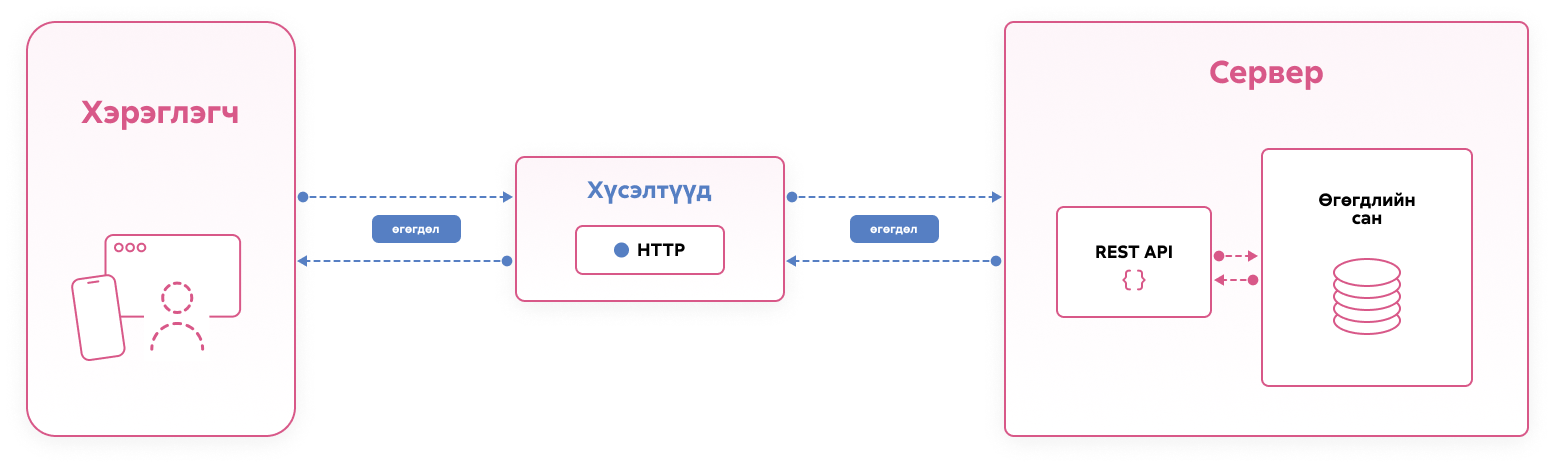
\includegraphics[width=15cm]{images/architecture.png}
	\caption{Client-Server Архитектурын үлгэр загварын дүрслэл}
	\label{fig:architecture}
\end{figure}

Хэрэглэгч талаас компьютер, гар утасны веб хөтчийг ашиглаж HTTP холболтоор хүсэлт явуулж, сервер талаас өгөгдлийн санг ашиглан REST API бэлдэн эргээд хэрэглэгч рүү HTTP холболтоор хүсэлтийн хариуг өгөх зарчмаар ажиллана.

\pagebreak
\section{Ажлын явцын диаграм}

\subsection{Ажлын явцын диаграм}
\begin{figure}[h]
	\centering
	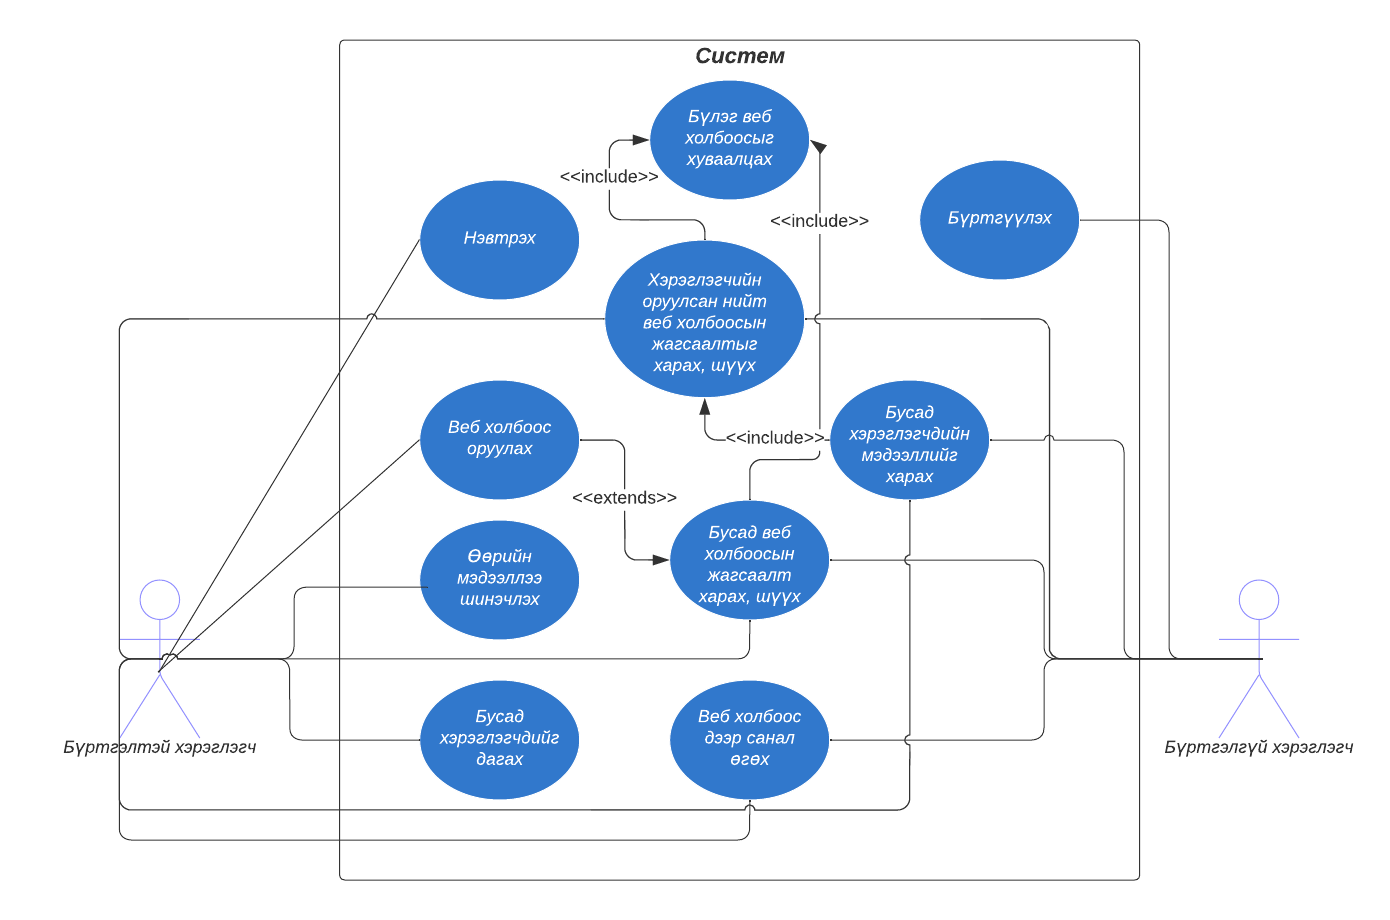
\includegraphics[width=15cm]{images/usecase.png}
	\caption{Ажлын явцын диаграм}
	\label{fig:usecase}
\end{figure}

\subsection{Ажлын явцын диаграмын тайлбар}

\begin{itemize}
	\item \textbf{Нэвтрэх -} Бүртгэлтэй хэрэглэгч өөрийн бүртгүүлсэн имэйл хаягаараа нэвтрэх, нууц үгээ сэргээх
	\item \textbf{Веб холбоос оруулах -} Өөрийн хүссэн веб холбоосоо дангаар нь болон бүлэглэж оруулах, хэрэв бүлэглэж оруулахаар бол тухайн бүлэг веб холбоосны нэр, тайлбаруудыг заавал авна
	\item \textbf{Өөрийн мэдээллээ шинэчлэх -} Өмнөх мэдээлэл хуучирсан эсвэл шинэчлэх шаардлага гарсан тохиолдолд хувийн мэдээлэл, холбооснуудынхаа нууцлалыг шинэчлэх
	\item \textbf{Бусад хэрэглэгчдийг дагах -} Өөрийн нүүр хуудсаа сонирхлынхоо дагуу хөгжүүлэхийг хүсвэл бусад хэрэглэгчдийг дагаж, тэдгээрийн оруулсан холбооснуудыг хамгийн эхэнд харах
	\item \textbf{Бусад веб холбоосын жагсаалтыг харах -} Систем дээр public байдлаар нийтлэгдсэн бүх веб холбоосыг шууд болон шүүсэн байдлаар харж өөрт хэрэгтэй мэдээллээ авах
	\item \textbf{Веб холбоос дээр санал өгөх -} Бүртгэлтэй болон бүртгэлгүй хэрэглэгчид тухайн веб холбоосны контентыг харсны дараагаар өөрийн хувийн саналаа өгч, чанарын үнэлгээ хийх 
	\item \textbf{Бүртгүүлэх -} Хэрэглэгч бүртгэлгүй хэдий ч манай платформыг бүрэн ашиглах боломжтой. Хэрэв өөрөө веб холбоос оруулахыг хүсвэл хувийн мэдээллээ бөглөж бүртгүүлэх
	\item \textbf{Хэрэглэгчийн оруулсан нийт веб холбоосын жагсаалтыг харах -} Зөвхөн нэг хэрэглэгчийн оруулсан private болон public веб холбооснуудыг нэг хуудсан харах, тэдгээрээс шүүх
	\item \textbf{Бусад хэрэглэгчдийн мэдээллийг харах -} Бүртгэлтэй болон бүртгэлгүй хэрэглэгч бусад хэрэглэгчдийн оруулсан хувийн мэдээллийг харах, холбоо барих мэдээллийг олох
	\item \textbf{Бүлэг веб холбоосыг хуваалцах -} Хэрэглэгч нэг сэдвийн хүрээнд олон веб холбоос оруулсан бол платформ дээр тухайн бүлгийн мэдээллийг харуулсан тусдаа нэг хуудас үүснэ. Түүний веб холбоосыг хуулж авах, бусад сошиал сүлжээнд түгээх
\end{itemize}

\pagebreak
\section{Өгөгдлийн сангийн диаграм}

\subsection{Өгөгдлийн сангийн диаграм}
\begin{figure}[h]
	\centering
	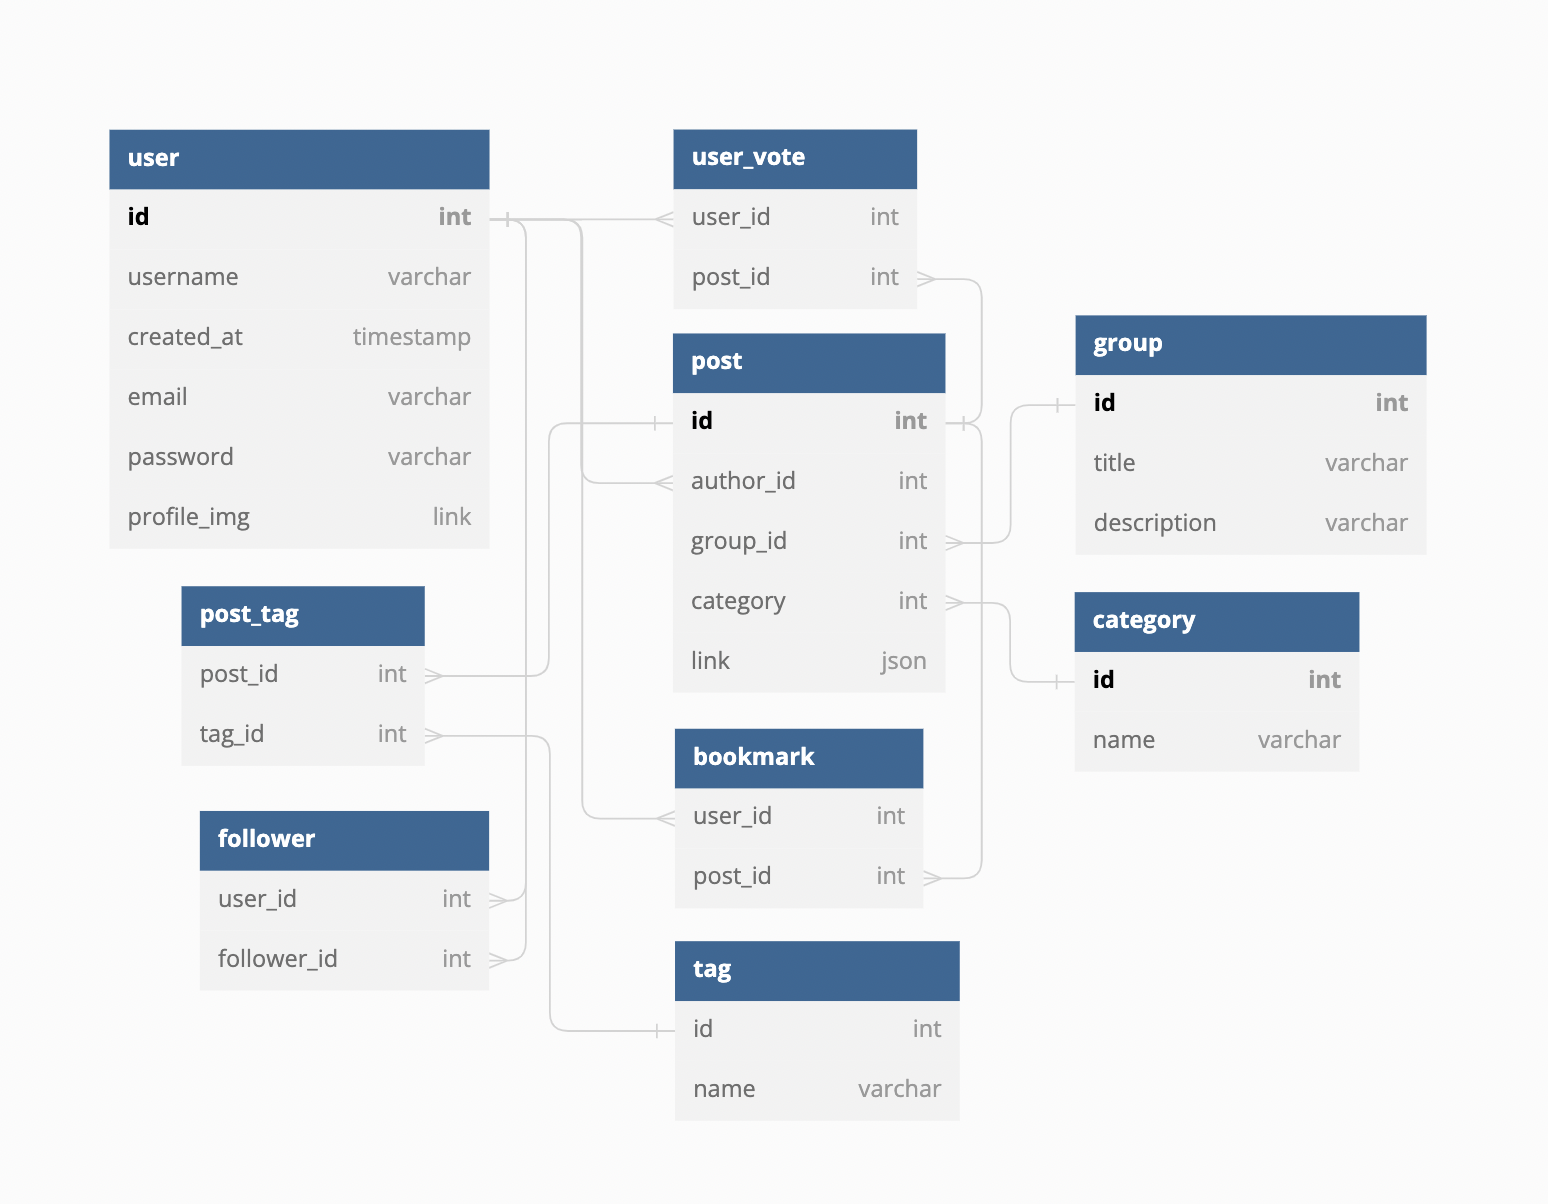
\includegraphics[width=15cm]{images/erdiagram.png}
	\caption{ER диаграм}
	\label{fig:erd}
\end{figure}

\subsection{Өгөгдлийн сангийн хүснэгтүүдийн тайлбар}

\begin{table}[h]
	\caption{user хүснэгт}
	\begin{tabular}{|l|l|l|p{8cm}|}
	\hline
	№ &  Талбарын нэр & Өгөгдлийн төрөл & Тайлбар \\ \hline
	1 &  id & int & Хэрэглэгчийн дахин давтагдашгүй ID-г хадгална - Auto Incremented \\ \hline
	2 &  username & varchar & Хэрэглэгчийн гараас оруулж өгсөн нэрийг хадгална. Зөвхөн латин тэмдэгтүүд ашиглах хэрэгтэй \\ \hline
	3 &  created\_at & timestamp & Хэрэглэгчийн хаяг үүссэн хугацааг серверээс авч хадгална \\ \hline
	4 &  email & varchar & Хэрэглэгчийн цахим шуудан \\ \hline
	5 &  password & varchar & Хэрэглэгчийн гараас оруулж өгсөн нууц үгийг encrypt-лэж уг хэсэгт хадгална \\ \hline
	6 &  profile\_img & link & Хэрэглэгчийн оруулж өгсөн зургийг сервер дээр хадгалж, замыг нь энэ хэсэгт хадгална \\ \hline

\end{tabular}
\end{table}

\begin{table}[h]
	\caption{post хүснэгт}
	\begin{tabular}{|l|l|l|p{8cm}|}
	\hline
	№ &  Талбарын нэр & Өгөгдлийн төрөл & Тайлбар \\ \hline
	1 &  id & int & Нийтлэлийн дахин давтагдашгүй ID-г хадгална - Auto Incremented \\ \hline
	2 &  author\_id & int & Тухайн нийтлэлийг бичсэн хэрэглэгчийн ID-г Foreign Key-р хадгална \\ \hline
	3 &  group\_id & int & Хэрэглэгч веб холбоосыг нэг дор олныг оруулах боломжтой ба тухайн тохиолдолд бүлэг веб холбоос гэж үзэн тухайн бүлгийн нэр, тайлбарыг хадгална \\ \hline
	4 &  category & int & Нийтлэлийн төрлийг хадгална. Нийтлэл дор хаяж нэг нийтлэлд харьяалагдах шаардлагатай \\ \hline
	5 &  link & json & Нэг болон түүнээс их холбоос хадгалах боломжтой болгож байгаа тул хэрэглэгчийн оруулж өгсөн веб холбоосуудыг уг талбарт json хэлбэрээр хадгална \\ \hline

\end{tabular}
\end{table}

\begin{table}[h]
	\caption{post\_tag хүснэгт}
	\begin{tabular}{|l|l|l|p{8cm}|}
	\hline
	№ &  Талбарын нэр & Өгөгдлийн төрөл & Тайлбар \\ \hline
	1 &  post\_id & int & Нэг нийтлэл хэдэн ч tag-тай байж болох ба уг талбарт нийтлэлийн ID-г Foreign Key-р авч ашиглаж байгаа \\ \hline
	2 &  tag\_id & int & Хэрэглэгч өөрсдөө Tag-аа үүсгэж өгөх боломжтой учир тухайн үүсгэсэн Tag-н ID-г авна \\ \hline

\end{tabular}
\end{table}

\begin{table}[h]
	\caption{follower хүснэгт}
	\begin{tabular}{|l|l|l|p{8cm}|}
	\hline
	№ &  Талбарын нэр & Өгөгдлийн төрөл & Тайлбар \\ \hline
	1 &  user\_id & int & Тухайн хэрэглэгчид хэнийг дагаж байгааг илэрхийлэх талбар \\ \hline
	2 &  follower\_id & int & Тухайн хэрэглэгчийг хэн дагаж байгааг илэрхийлэх талбар \\ \hline

\end{tabular}
\end{table}

\begin{table}[h]
	\caption{user\_vote хүснэгт}
	\begin{tabular}{|l|l|l|p{8cm}|}
	\hline
	№ &  Талбарын нэр & Өгөгдлийн төрөл & Тайлбар \\ \hline
	1 &  user\_id & int & Хэн тухайн нийтлэл дээр санал өгсныг хадгалах талбар \\ \hline
	2 &  post\_id & int & Тухайн хэрэглэгч аль нийтлэл дээр санал өгсныг хадгалах талбар \\ \hline

\end{tabular}
\end{table}

\begin{table}[h]
	\caption{group хүснэгт}
	\begin{tabular}{|l|l|l|p{8cm}|}
	\hline
	№ &  Талбарын нэр & Өгөгдлийн төрөл & Тайлбар \\ \hline
	1 &  id & int & Primary Key бөгөөд хэрэглэгч олон веб холбоос оруулж өгөх боломжтой. Үүнийг бид бүлэг холбоос гэж нэрлэж байгаа ба энэ тохиолдолд тухайн бүлэгт заавал нэр болон тайлбар утга байх хэрэгтэй \\ \hline
	2 &  title & varchar & Бүлэг холбоосын гарчгийг хадгалах талбар \\ \hline
	3 &  description & varchar & Бүлэн холбоосын тайлбарыг хадгалах талбар \\ \hline

\end{tabular}
\end{table}

\begin{table}[h]
	\caption{category хүснэгт}
	\begin{tabular}{|l|l|l|p{8cm}|}
	\hline
	№ &  Талбарын нэр & Өгөгдлийн төрөл & Тайлбар \\ \hline
	1 &  id & int & Primary Key бөгөөд хэрэглэгч нийтлэлийн төрөл олон байх боломжтой. \\ \hline
	2 &  name & varchar & Төрлийн нэрийг хадгалах талбар \\ \hline

\end{tabular}
\end{table}

\begin{table}[h]
	\caption{bookmark хүснэгт}
	\begin{tabular}{|l|l|l|p{8cm}|}
	\hline
	№ &  Талбарын нэр & Өгөгдлийн төрөл & Тайлбар \\ \hline
	1 &  user\_id & int & Хэрэглэгч өөрт таалагдсан нийтлэлээ хадгалах шаардлагатай ба уг талбарт тухайн нийтлэлийг хадгалсан хэрэглэгчийн ID-г Foreign Key-р хадгална \\ \hline
	2 &  post\_id & int & Хэрэглэгчийн хадгалсан нийтлэлийн ID-г хадгална \\ \hline

\end{tabular}
\end{table}

\begin{table}[h]
	\caption{tag хүснэгт}
	\begin{tabular}{|l|l|l|p{8cm}|}
	\hline
	№ &  Талбарын нэр & Өгөгдлийн төрөл & Тайлбар \\ \hline
	1 &  id & int & Хэрэглэгчийн гараас оруулж өгсөн tag-н ID-г хадгална - Auto Incremented \\ \hline
	2 &  name & int & Хэрэглэгчийн гараас оруулж өгсөн tag-н нэрийг уг талбарт хадгална \\ \hline

\end{tabular}
\end{table}


\clearpage
\section{Хэрэглэгчийн интерфейс дизайн}

Өмнөх бүлэгт хийсэн UX судалгаан дээрээ үндэслэж User Experience болон User Interface загварыг High Fidelity түвшинд эцэслэж гаргасан ба гаргасан дизайнаа хэрэглэгчээр туршиулж тодорхой үр дүнгүүдэд хүрч чадсан. Үүнд: 

\begin{itemize}
	\item Хэрэглэгчийн шаардлагыг бүрэн ойлгож, хэрэглэгч суурьтай дизайн гаргасан
	\item Тусдаа бүлэг ажил болгон хийснээр интерфейс загвартаа анхаарч шинэлэг, ойлгомжтой интерфейс бүтээсэн
	\item Хөгжүүлэлтийн шатнаас өмнө бүх интерфейсүүд дизайн системийн дагуу гарч дууссан тул front-end хөгжүүлэлтийн явцыг илт хурдлуулсан
	\item Интерфейсийн дагуу front-end код явагдах тул back-end код дээр dummy датагаар хөгжүүлж явах, төлөвлөх үе шат хялбар болсон. Front-end хэсэгтэй зөрөх магадлал багассан гэж ойлгож болно.
\end{itemize}

\begin{figure}[h]
	\centering
	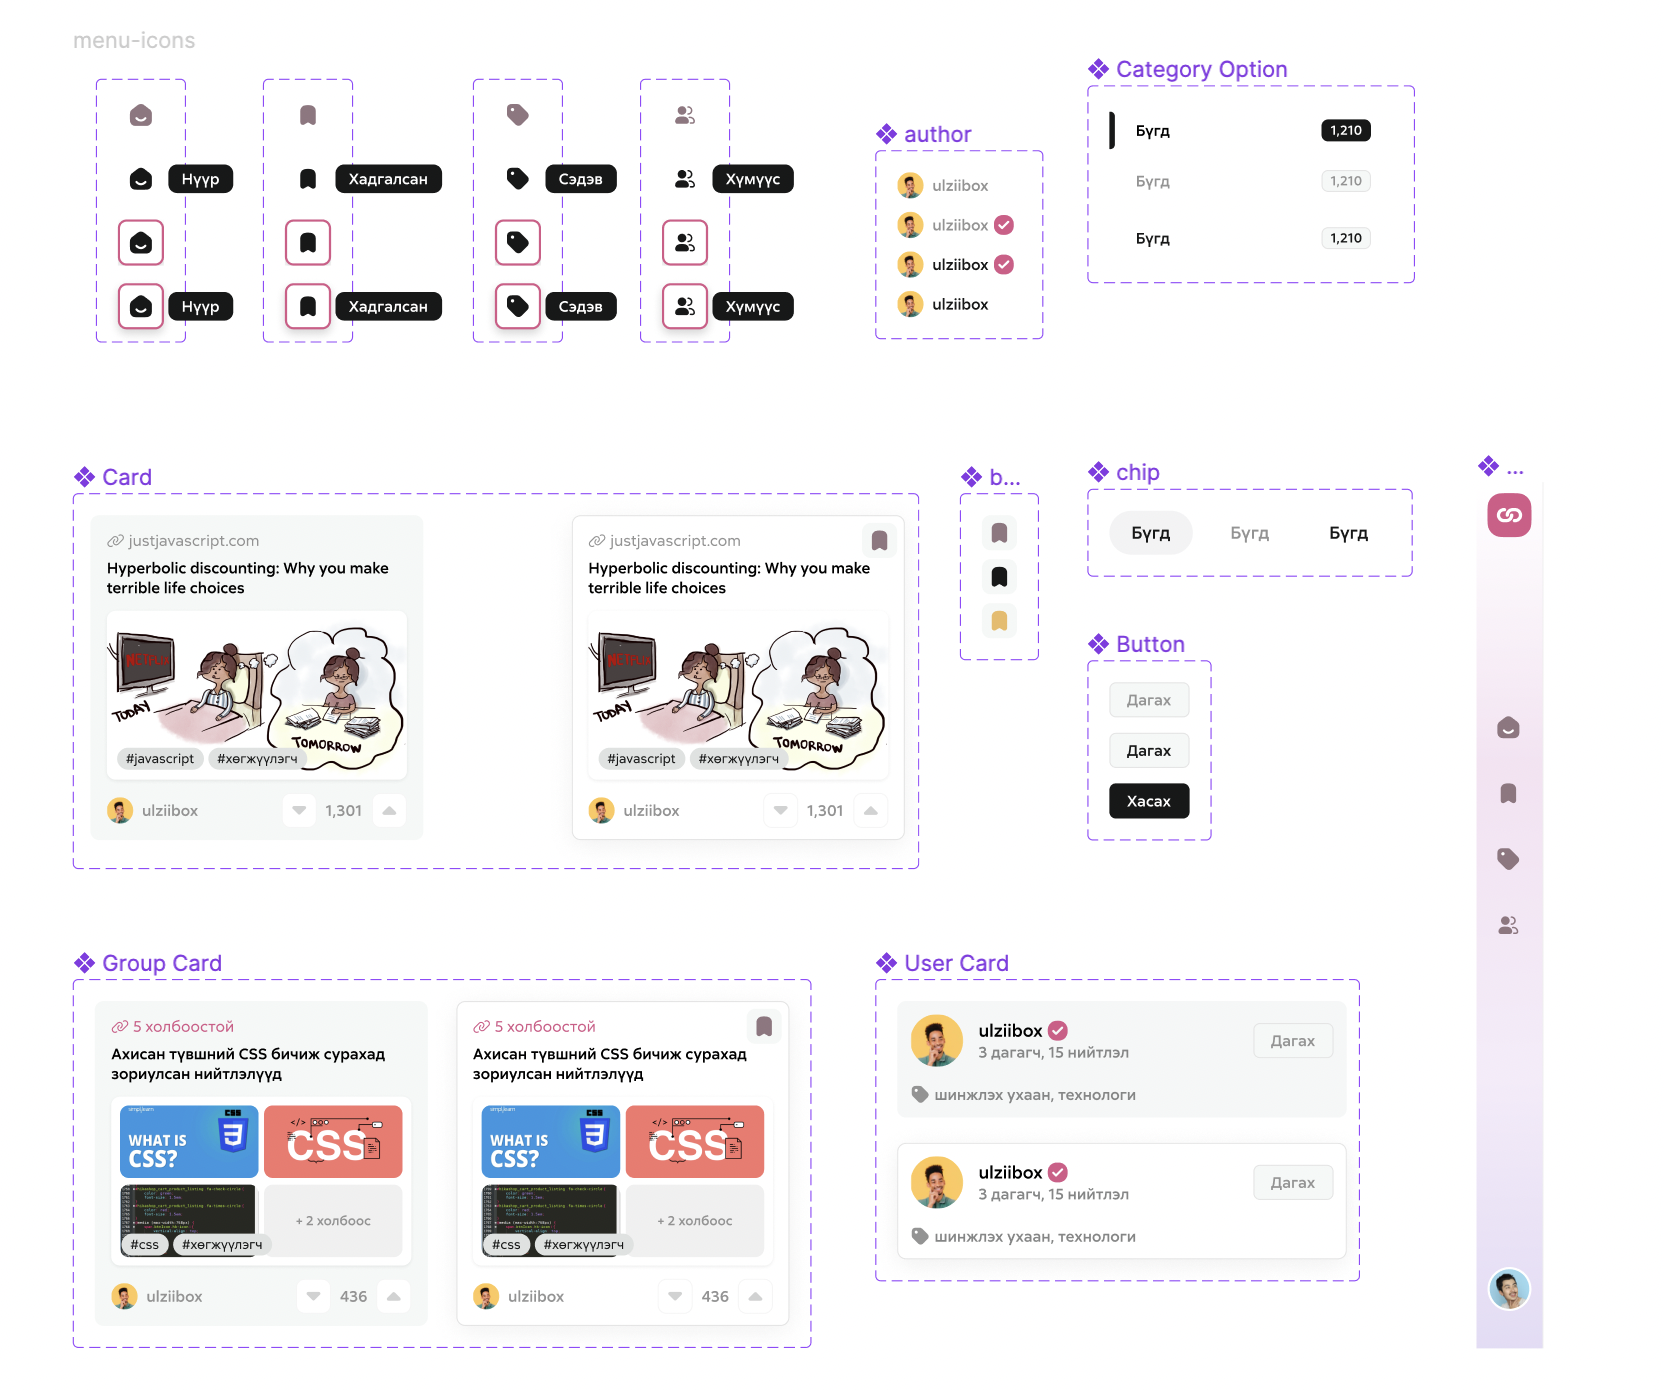
\includegraphics[width=15cm]{images/interfaces/components.png}
	\caption{Ашигласан компонентуудын жишээ}
	\label{fig:component}
\end{figure}

\begin{figure}[h]
	\centering
	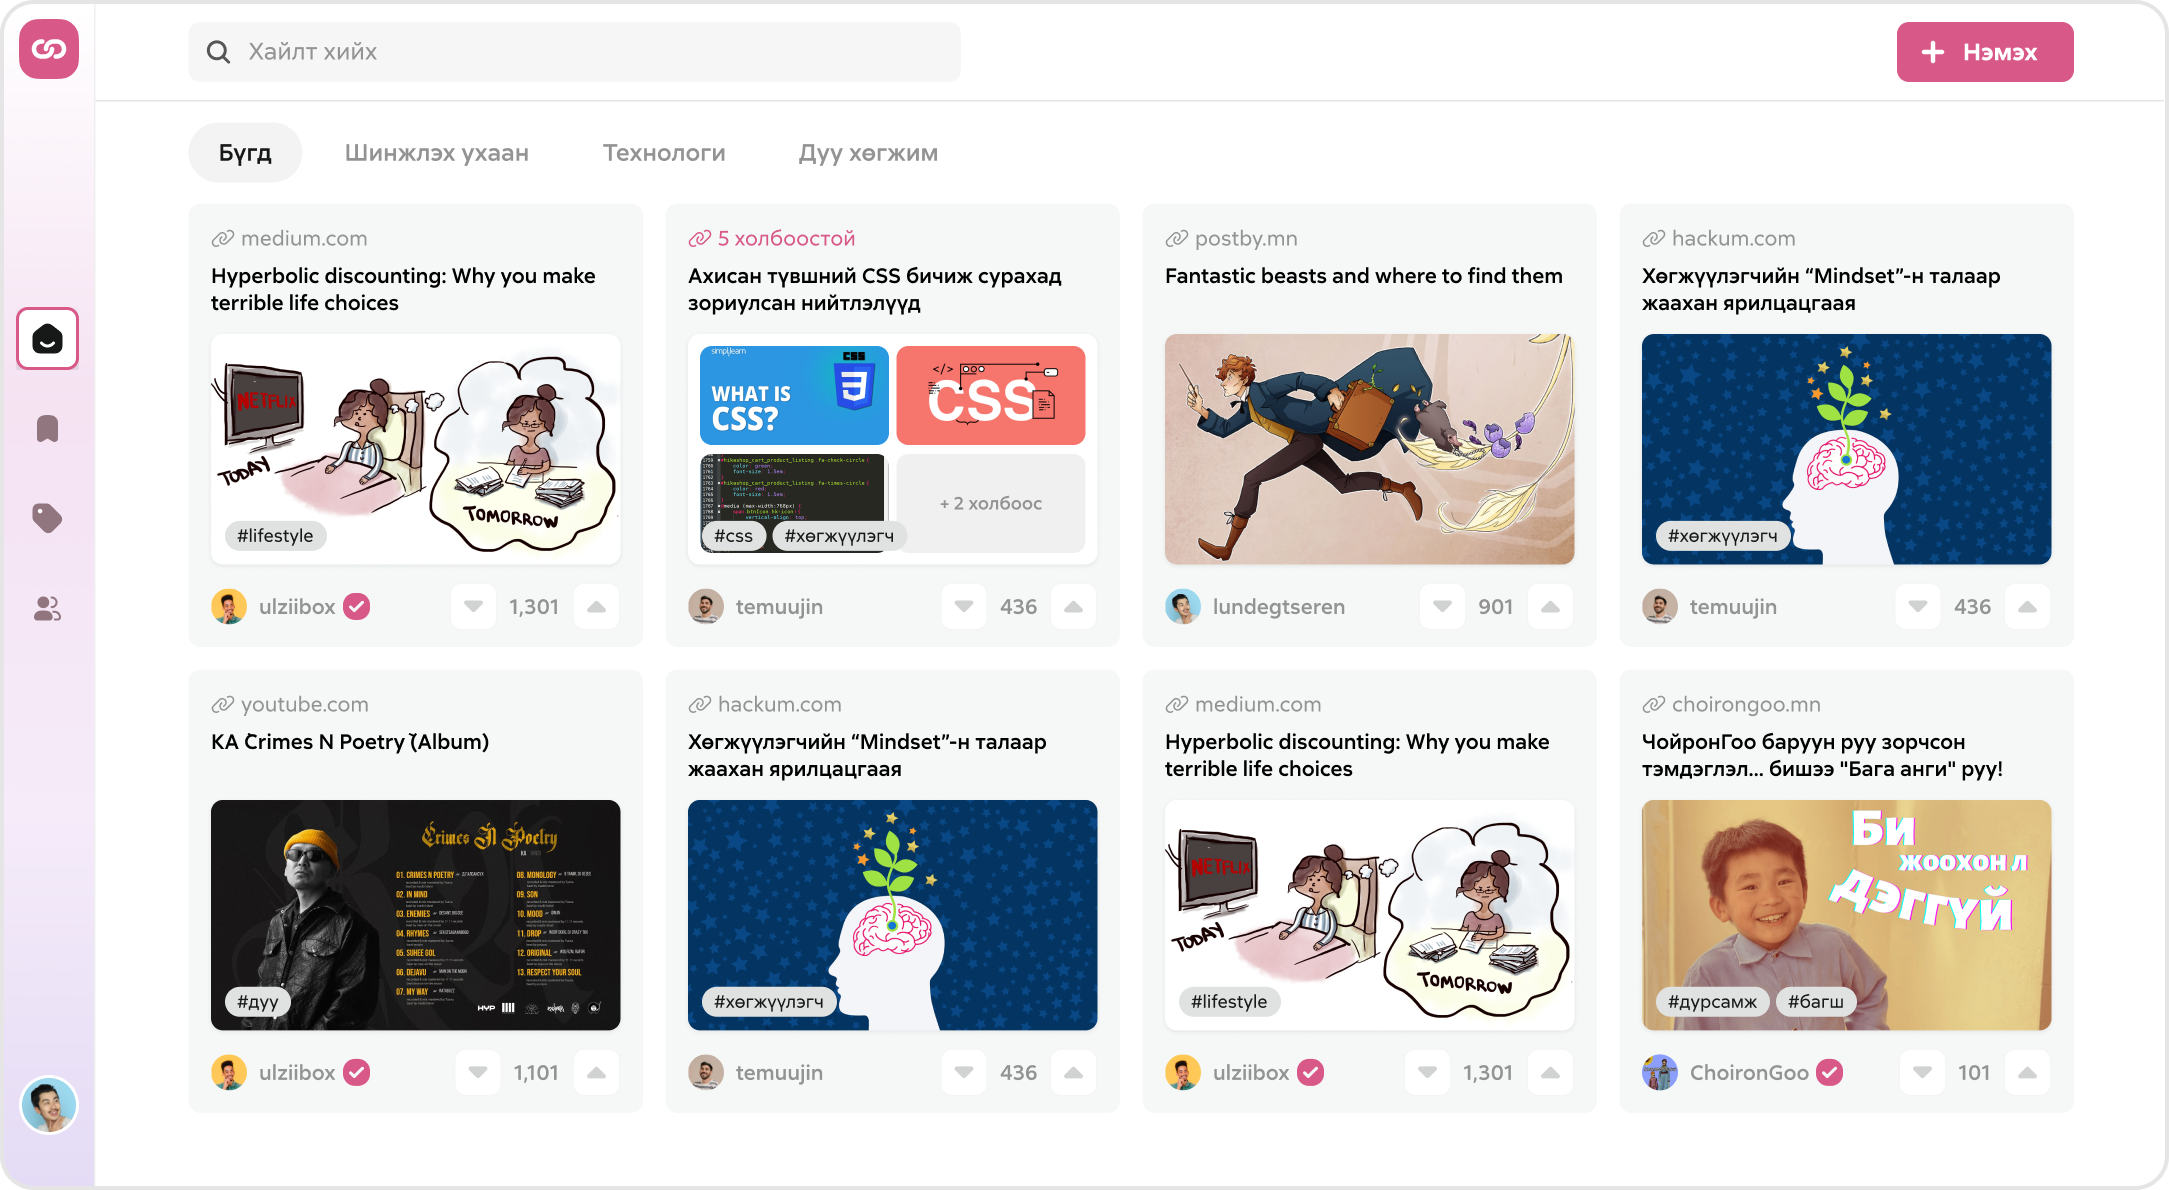
\includegraphics[width=15cm]{images/interfaces/home-screen.png}
	\caption{Нэвтэрсний дараах нүүр хуудас}
	\label{fig:homescreen}
\end{figure}

\begin{figure}[h]
	\centering
	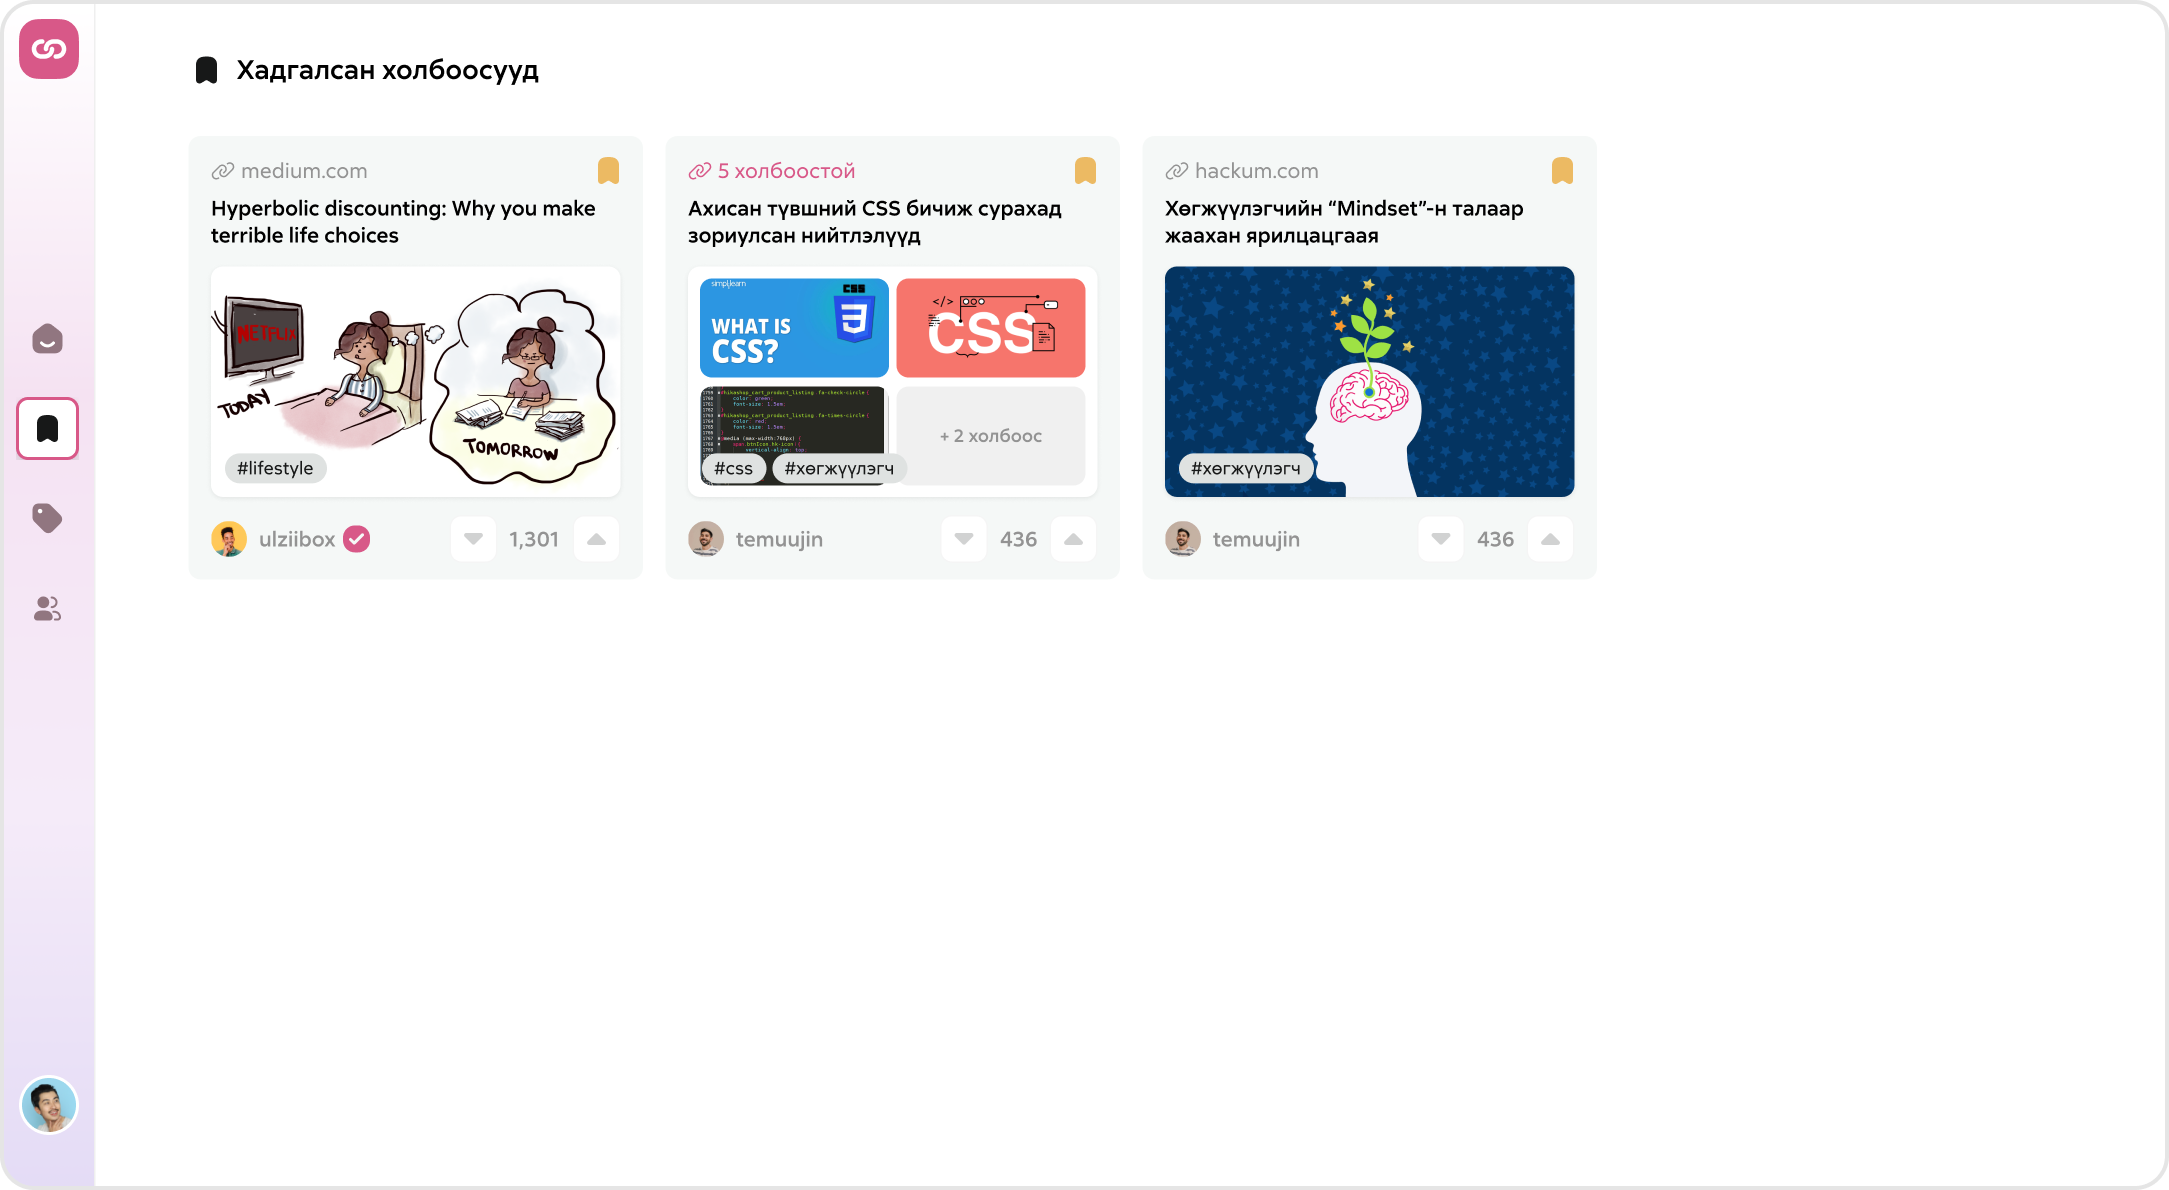
\includegraphics[width=15cm]{images/interfaces/bookmark.png}
	\caption{Хадгалсан холбоосуудын жагсаалт}
	\label{fig:bookmark}
\end{figure}

\begin{figure}[h]
	\centering
	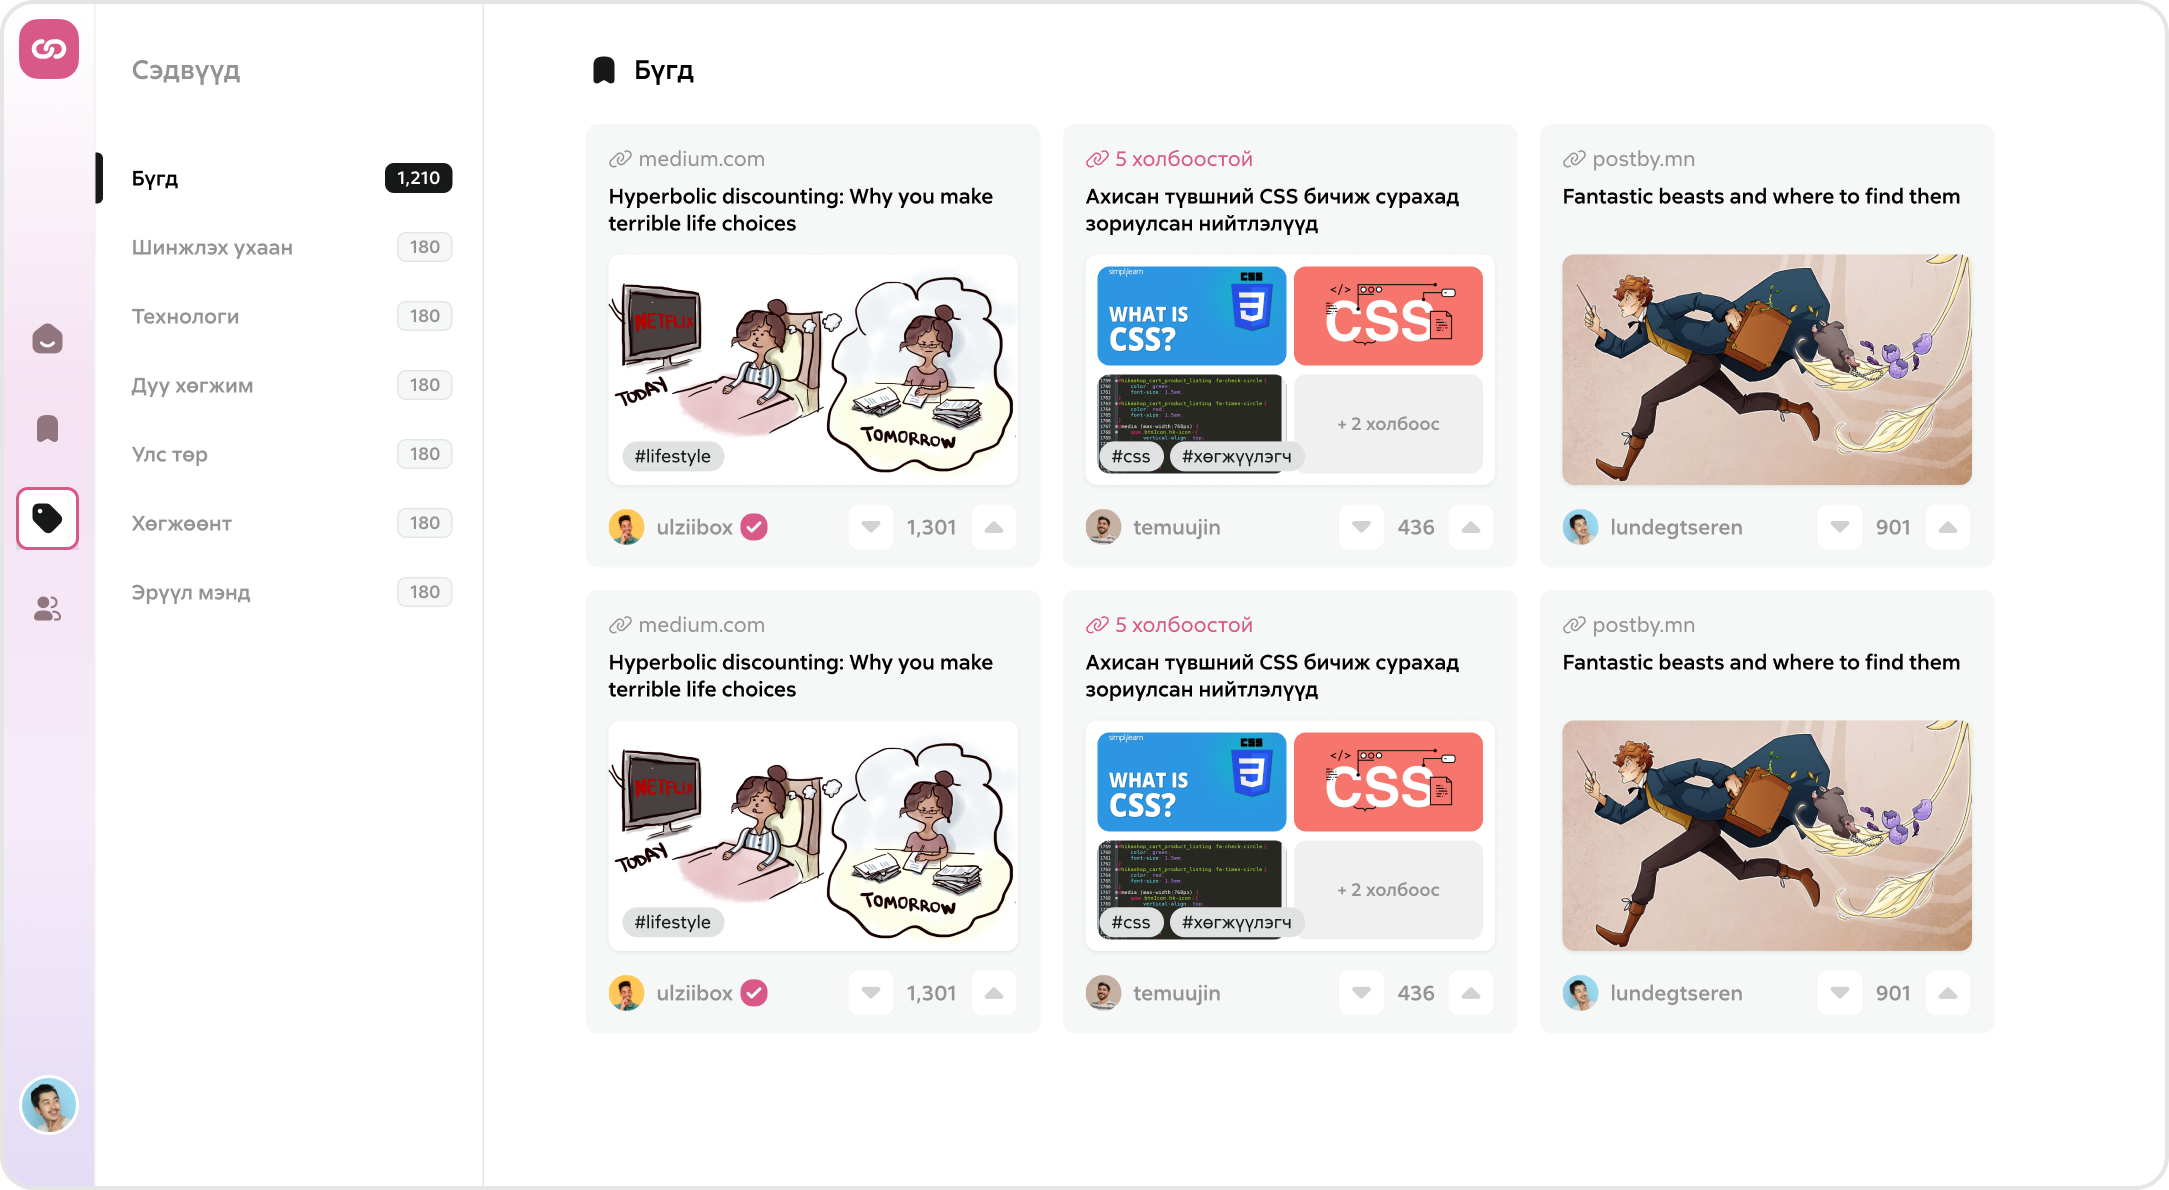
\includegraphics[width=15cm]{images/interfaces/topics.png}
	\caption{Бүх холбоосуудыг төрлөөр нь шүүж харах хуудас}
	\label{fig:topics}
\end{figure}

\begin{figure}[h]
	\centering
	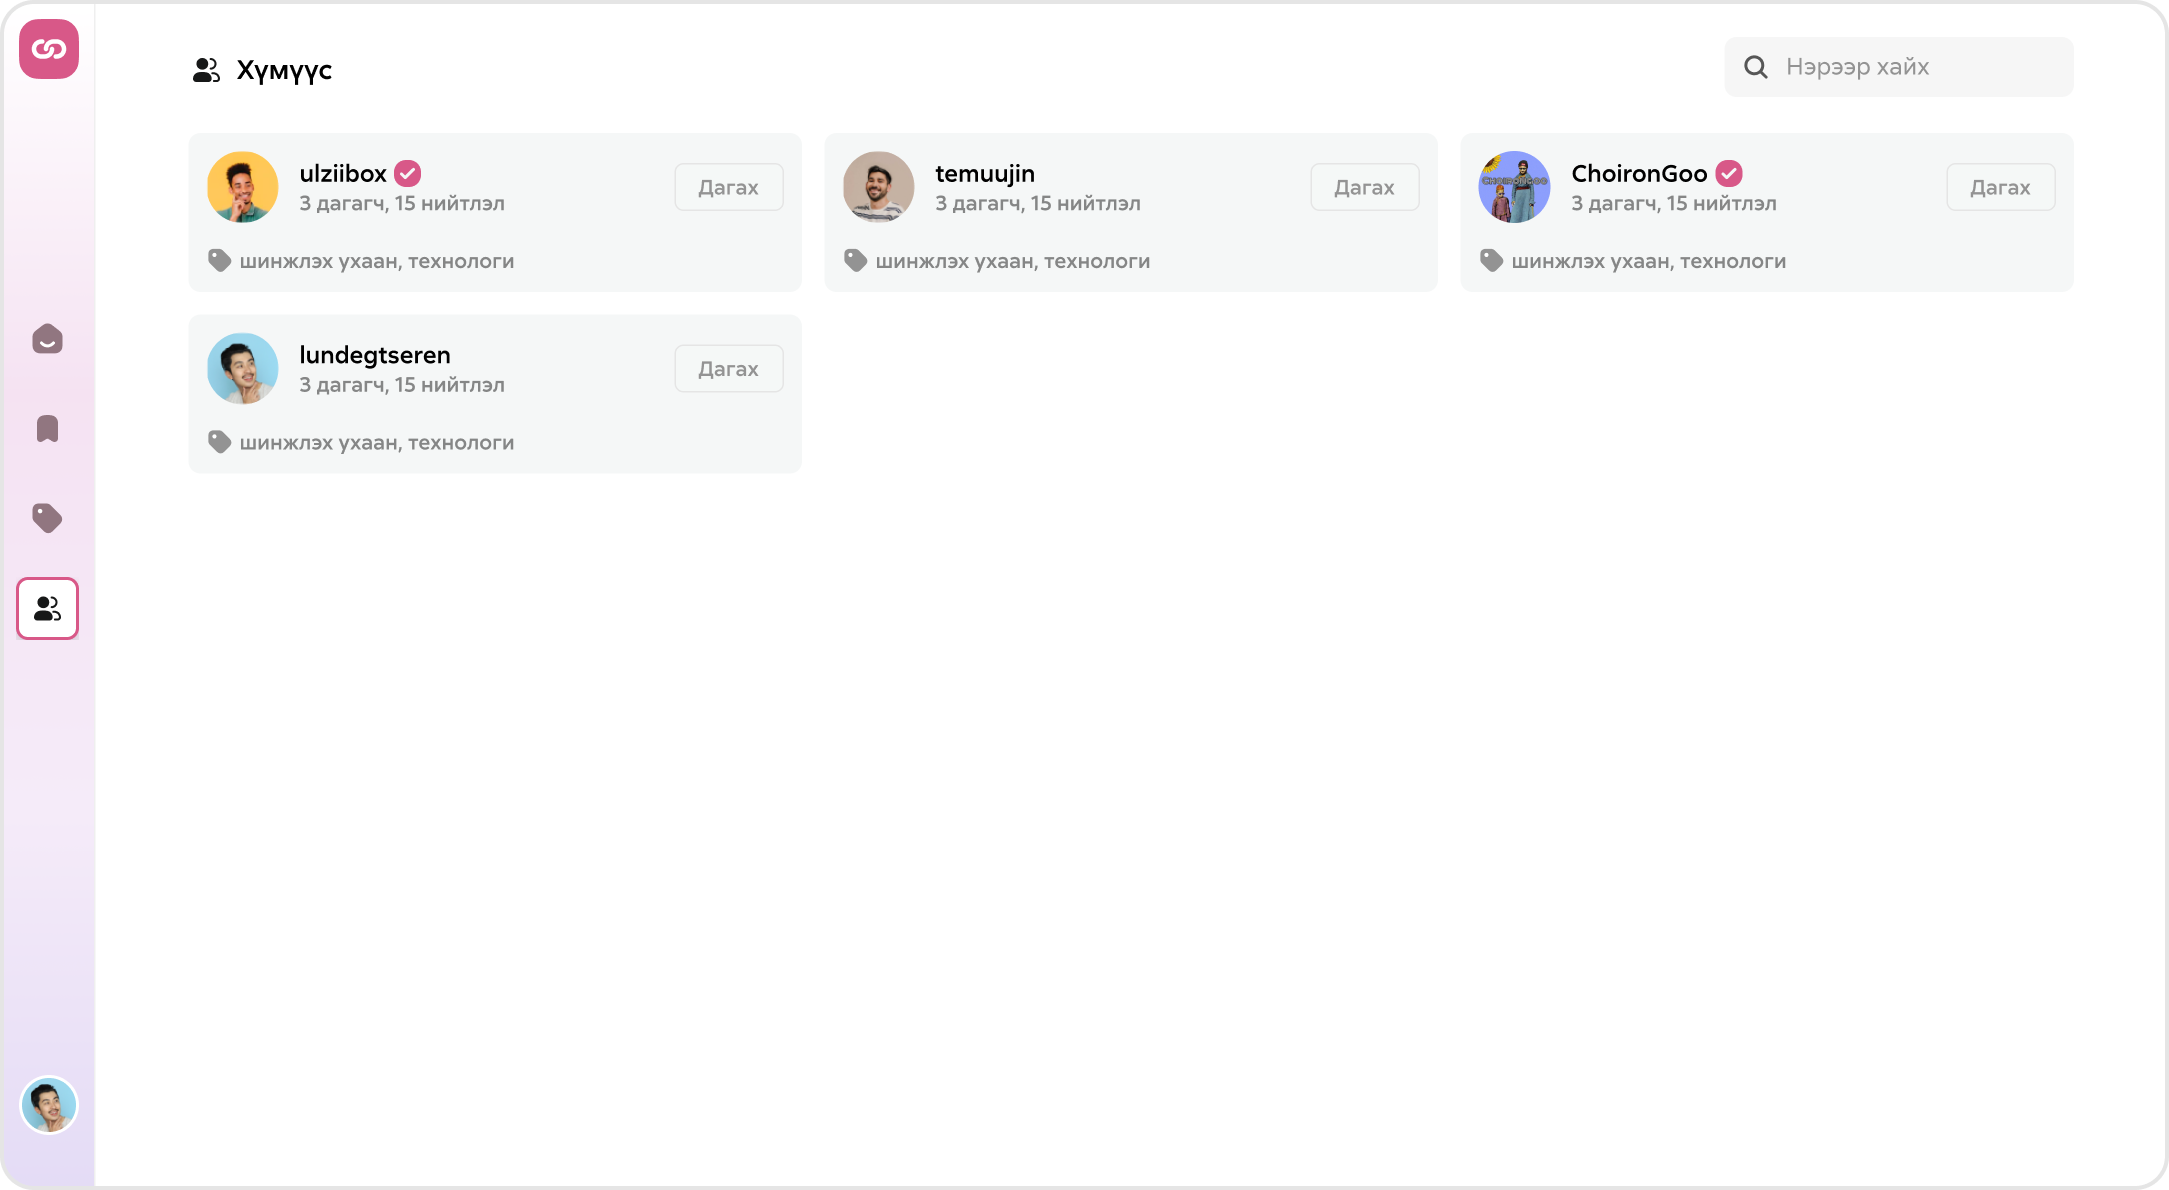
\includegraphics[width=15cm]{images/interfaces/people.png}
	\caption{Хэрэглэгчдийн жагсаалт харагдах хуудас}
	\label{fig:people}
\end{figure}

\begin{figure}[h]
	\centering
	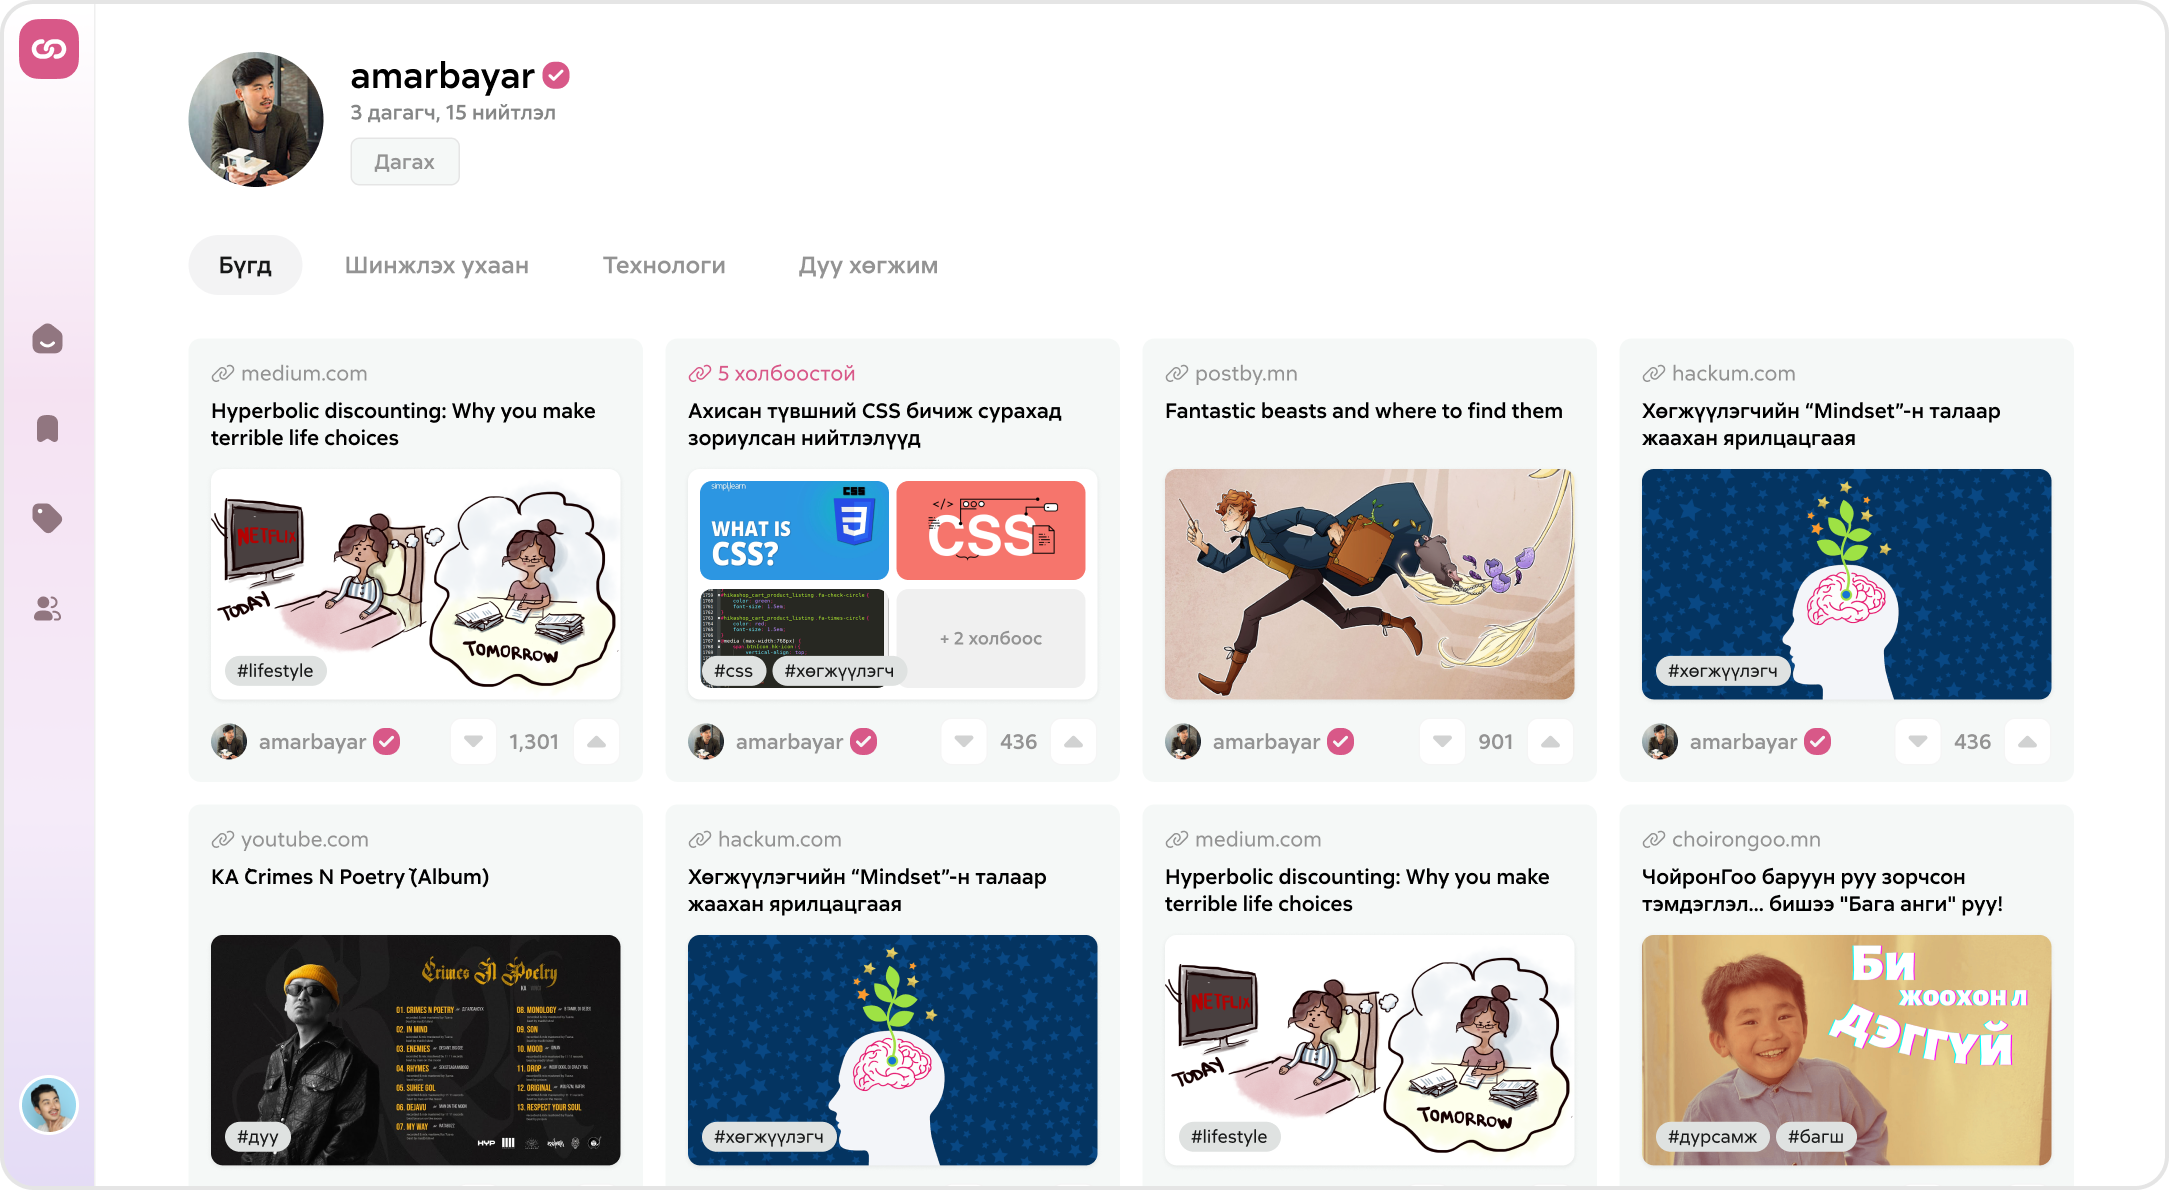
\includegraphics[width=15cm]{images/interfaces/profile.png}
	\caption{Бусдын профайлыг харах хуудас}
	\label{fig:profile}
\end{figure}

\begin{figure}[h]
	\centering
	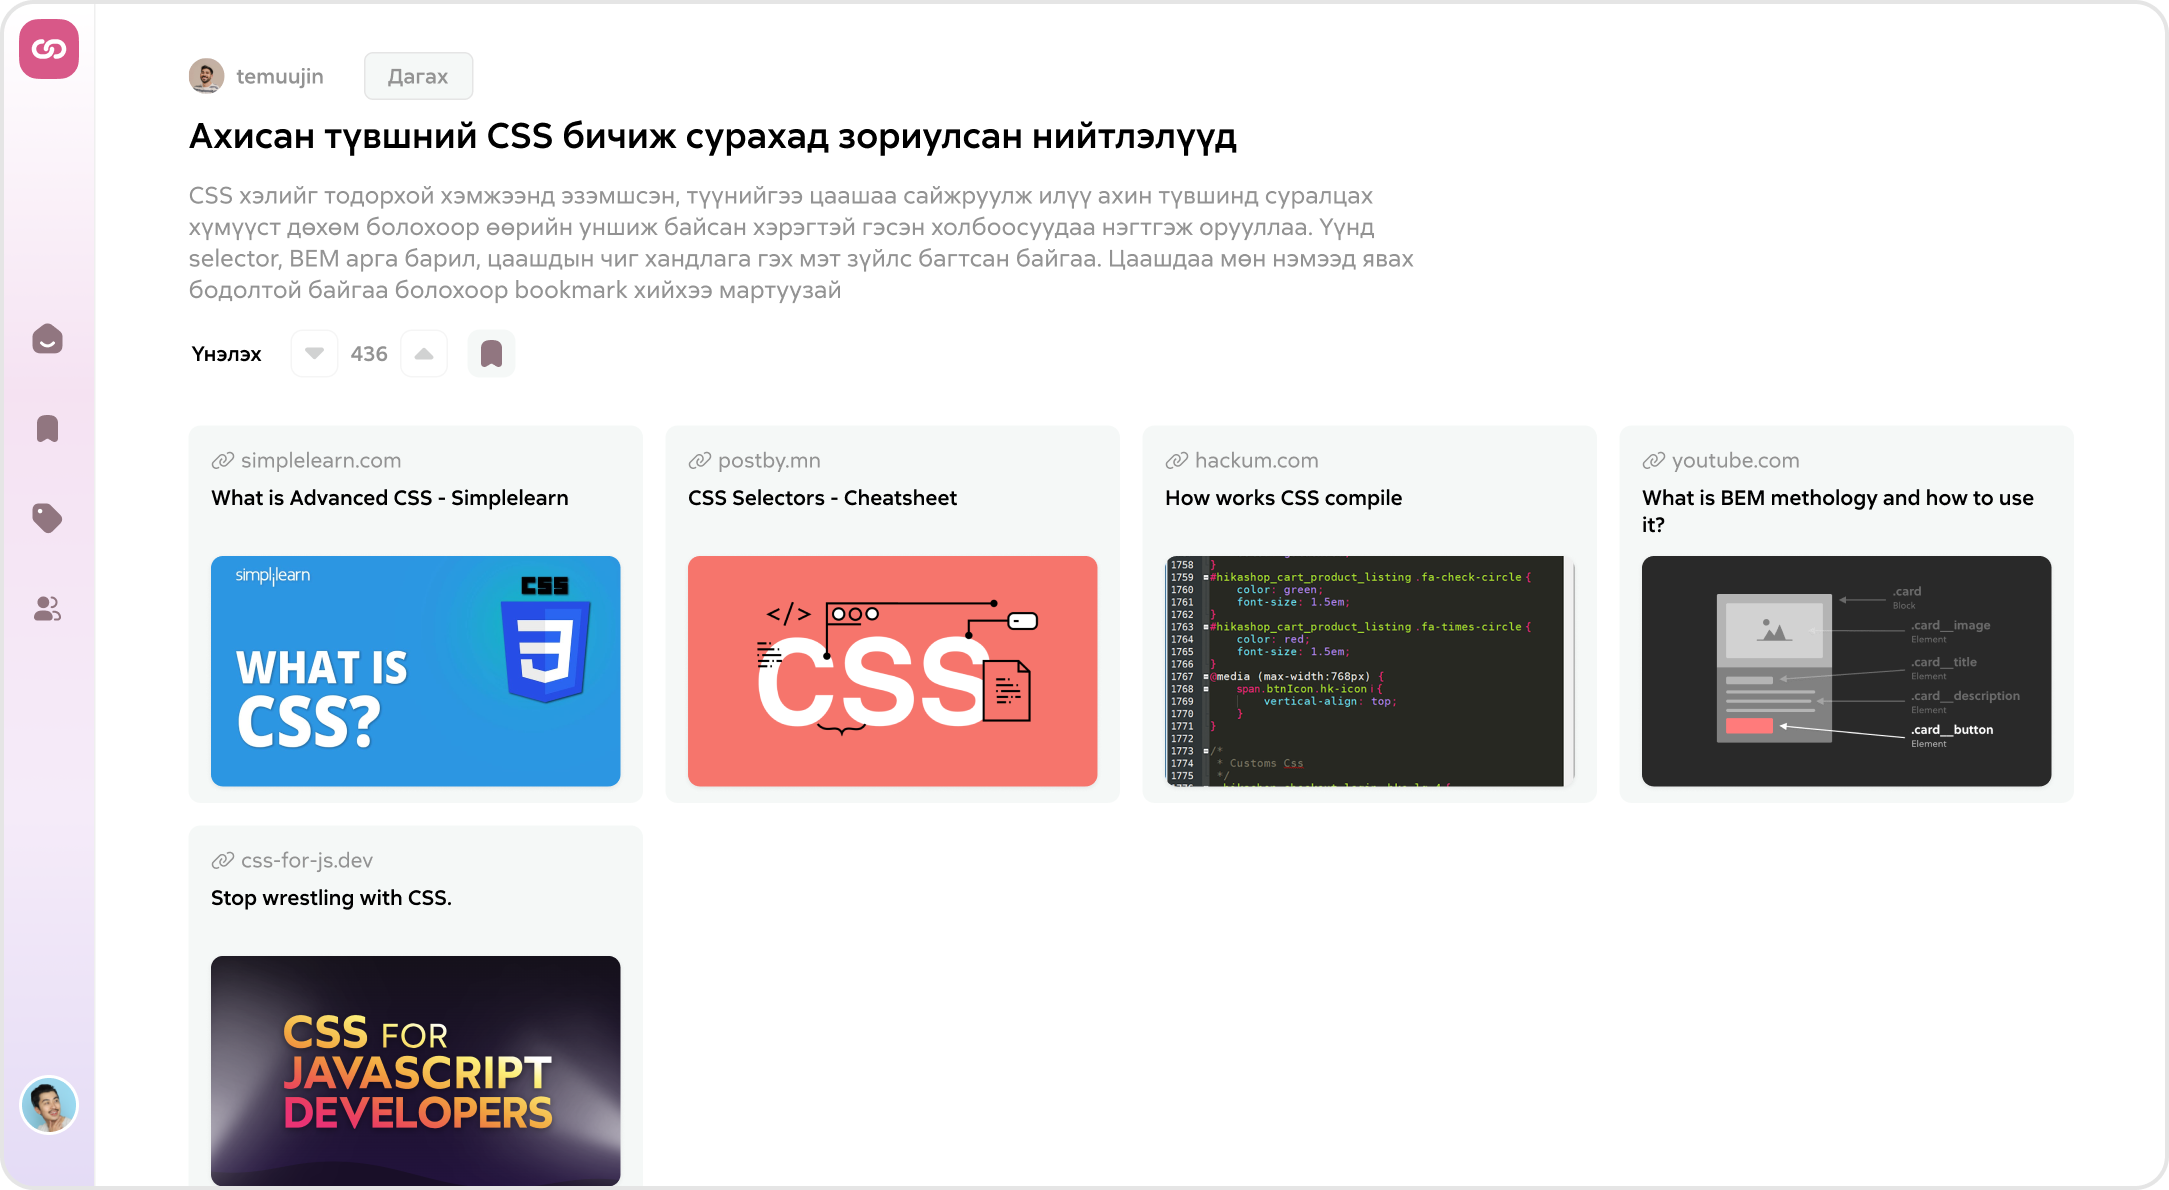
\includegraphics[width=15cm]{images/interfaces/grouped-link.png}
	\caption{Бүлэг холбоос доторх холбоосуудыг харах хуудас}
	\label{fig:grouped}
\end{figure}






